
\documentclass[]{standalone}

\usepackage[english]{babel}
\usepackage{amsmath}
\usepackage{amssymb}
\usepackage{graphicx}
\usepackage{xspace}
\usepackage{booktabs}
\usepackage{xcolor}
\setlength\parindent{0pt}

\begin{document}
\begin{tabular}{c}
$ U = e^{iH_{0}} $, canonical, trotter steps = 1, 2, 4, 8 \\
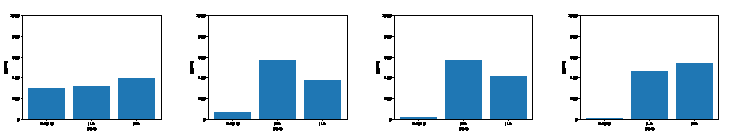
\includegraphics[width=1.0\textwidth]{col_d_0_r_0_rc_0_steps_1_2_4_8.pdf} \\
$ U = e^{iH_{0}} $, randomize, trotter steps = 1, 2, 4, 8 \\
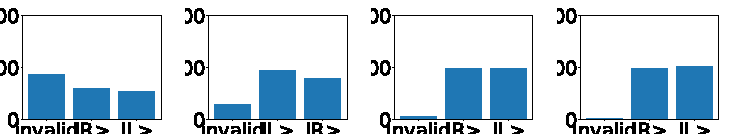
\includegraphics[width=1.0\textwidth]{col_d_0_r_1_rc_0_steps_1_2_4_8.pdf} \\
$ U = e^{iH_{1}} $, canonical, trotter steps = 1, 2, 4, 8 \\
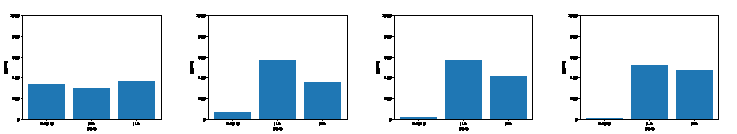
\includegraphics[width=1.0\textwidth]{col_d_1_r_0_rc_0_steps_1_2_4_8.pdf} \\
$ U = e^{iH_{1}} $, randomize, trotter steps = 1, 2, 4, 8 \\
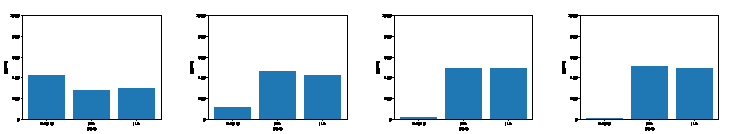
\includegraphics[width=1.0\textwidth]{col_d_1_r_1_rc_0_steps_1_2_4_8.pdf} \\
$ U = e^{i\frac{H_{0}}{2}}e^{i\frac{H_{1}}{2}} $, canonical, trotter steps = 1, 2, 4, 8 \\
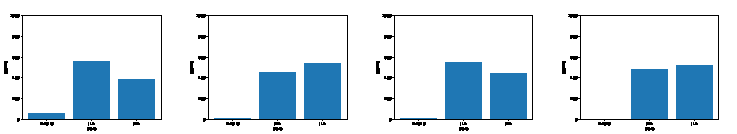
\includegraphics[width=1.0\textwidth]{col_d_2_r_0_rc_0_steps_1_2_4_8.pdf} \\
$ U = e^{i\frac{H_{0}}{2}}e^{i\frac{H_{1}}{2}} $, randomize, trotter steps = 1, 2, 4, 8 \\
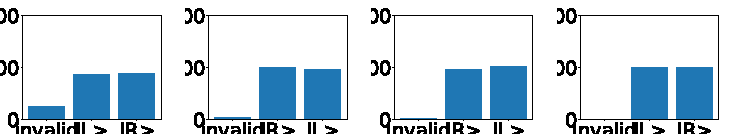
\includegraphics[width=1.0\textwidth]{col_d_2_r_1_rc_0_steps_1_2_4_8.pdf} \\
$ U = e^{i\frac{H_{0}}{2}}e^{i\frac{H_{1}}{2}} $, randomize unitaries, trotter steps = 1, 2, 4, 8 \\
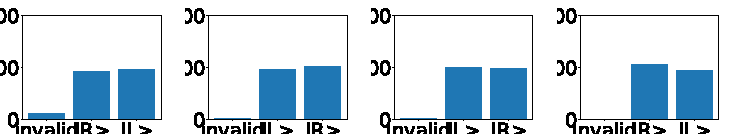
\includegraphics[width=1.0\textwidth]{col_d_2_r_0_rc_1_steps_1_2_4_8.pdf} \\
\end{tabular}
\end{document}
